\documentstyle[12pt, epsfig]{article} 

\title{The SLAM+(ERSEM+POLCOMS) model coupling }
\author{Asbj{\o}rn Christensen \\ DTU Aqua \\ MEECE deliverable 2.11}

\begin{document}
\maketitle  

% ===================================================
\section{Introduction}
% ===================================================

This document contains a short description and user guide 
of the SLAM (Sandeel Larval Advection model) model, 
coupled offline with the POLCOMS+ERSEM model
provided by Plymouth Marine Laboratory (PML) in the MEECE project. 
The SLAM model underlying this implementation is published
mainly in Can. J. Fish. Aquat. Sci. 65: 1498-1511 (2008) by Christensen {\em et al}.
  
The SLAM in the present implementation is set up within
the IBMlib (Individual based model library) framework maintained by DTU Aqua.
The present code package, however, contains only a self contained subset of the IBMlib
framework. The basic idea of IBMlib is sketched
% ----------------------------------------------------------------------------
\begin{figure}[p]   % [tbhp]
\begin{center}                                                  %% NO_WC_WOUNT
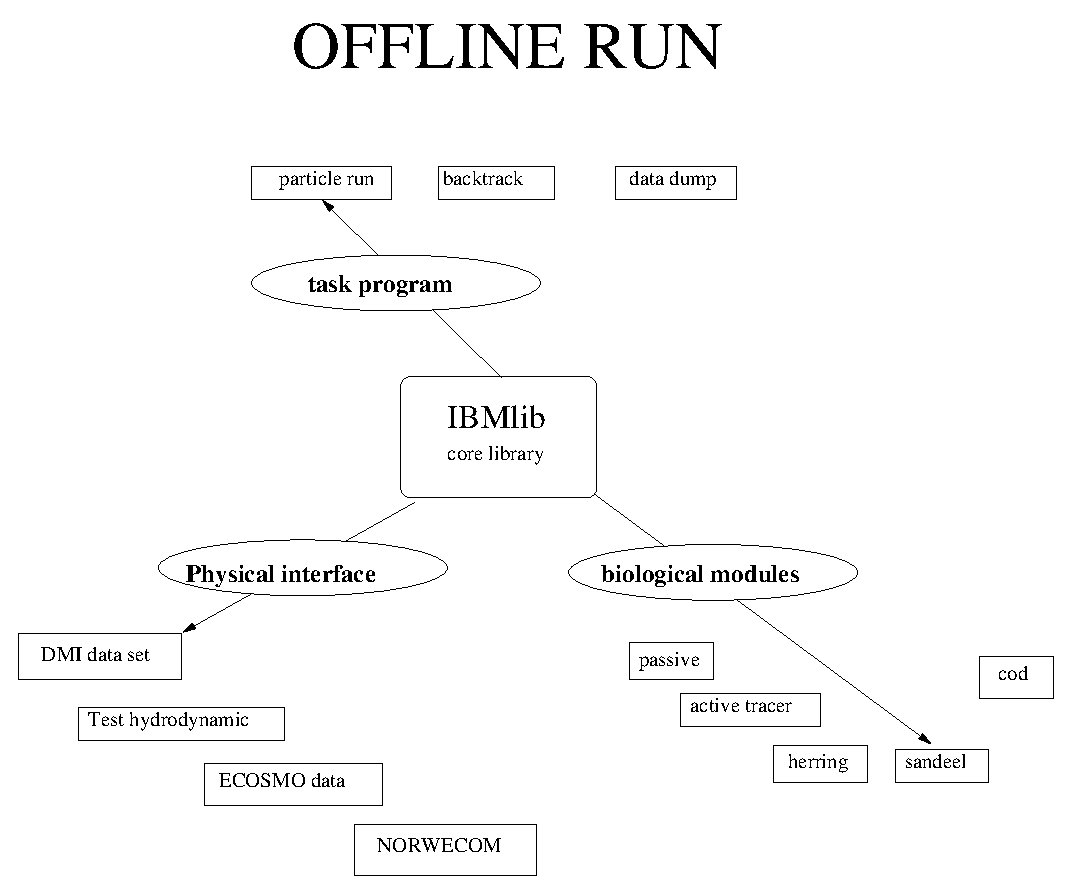
\epsfig{file=IBMlib_offline.eps,width=120mm,angle=0,clip=}     %% NO_WC_WOUNT
%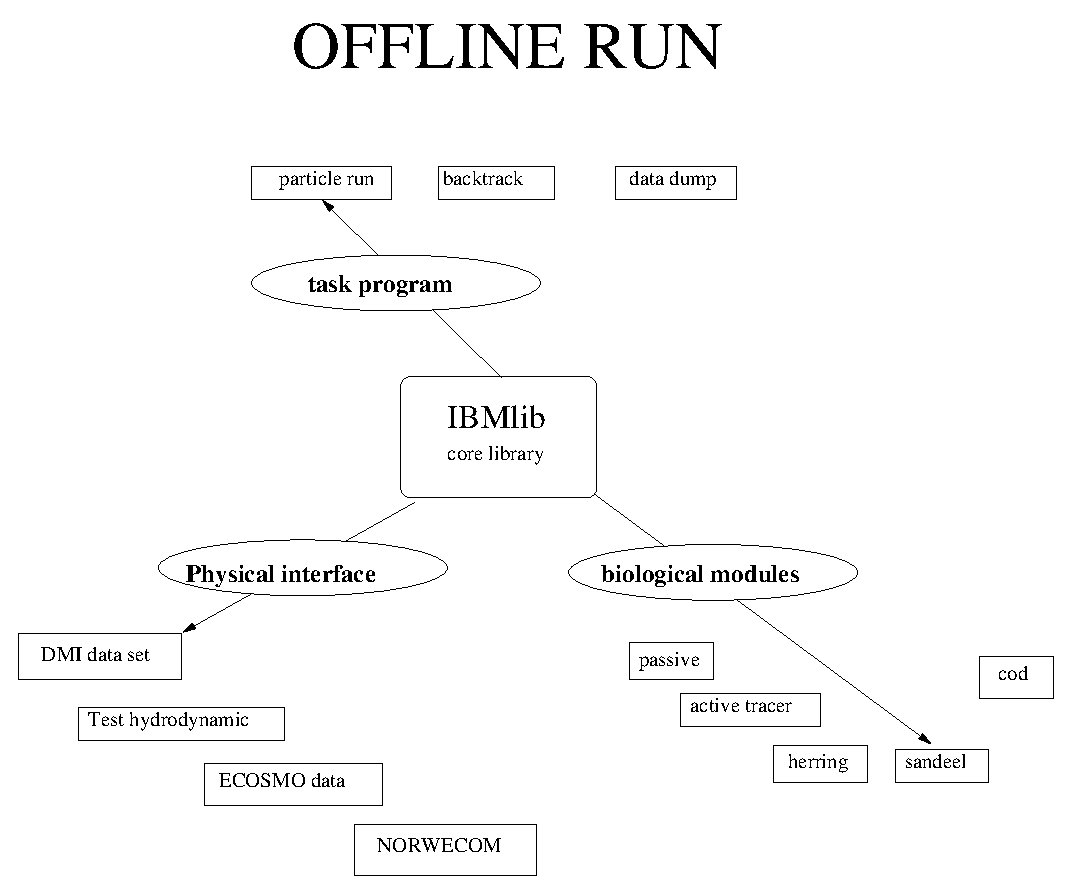
\includegraphics[width=120mm]{IBMlib_offline.eps}     %% NO_WC_WOUNT
\end{center}                                                    %% NO_WC_WOUNT
\caption{Concept diagram of the IBMlib framework.}
\label{cmp1Dvs2D}
\end{figure}
% ----------------------------------------------------------------------------
and is very well in line with the goal of MEECE to ease the traditionally cumbersome 
process of coupling biological models to arbitrary biogeochemical models.
The present code package is a preliminary demonstration coupling of the SLAM and 
POLCOMS+ERSEM models; the production runs in MEECE WP 3+4 will be performed with an
upgraded and extended version of the present code package, and interested MEECE
participants are encouraged to obtain latest version before embarking on simulations
on their own with the SPAM model setup.
 
% ===================================================
\section{Functionality}
% ===================================================

SLAM+(POLCOMS+ERSEM) setup allows you to perform flexible individual-based modelling
of early life stages within the space-time window covered be a supplied POLCOMS+ERSEM
data set. Sandeel larvae and/or eggs can be released according to any space-time pattern
specified in the input file. The model describes growth of egg/larvae in relation to
local physical conditions obtained from the supplied POLCOMS+ERSEM data set. The model 
can easily be extended by alternative biological processes, e.g. alternative 
active larval behavior.

% ===================================================
\section{License and intellectual property rights}
% ===================================================

At some point it is planned to make the IBMlib public available, but
this awaits the clarification of some the license issues of integrated 
external packages as well as code hosting and distribution issues; until
then, the code is available to MEECE participants within the MEECE project
under provisions specified in the MEECE consortium agreement and the 
intellectual property rights belong to DTU Aqua.

% ===================================================
\section{Installation}
% ===================================================

\subsection{Portability} 
The code is written in strict Fortran 90 and does not 
invoke operating system specific features nor does the 
code rely on non-standard compiler specific services.
Therefore the code (possibly with some surficial preparations)
should compile and execute on any platform; however, the
code has only been applied on Linux platforms until now.

\subsection{Requirements} 

In order to build the SLAM executable, the following resources must be
available:

\begin{itemize}
  \item A Fortran 90+ compiler and C++ compiler. The compiler and link flags
        in the Makefile applies to Intels {\em ifort} compiler,
        however the transcription of of these flags should be
        straightforward by consulting the documentation of 
        alternative compilers; most flags are standardized.
         
  \item NetCDF. The code assumes the Fortran 90 implementation
        (the fortran-only variant) is installed (at compilation time by use association of
        of the netcdf module - usually netcdf.mod, somewhere in the 
        include path - and at link time by linking to libnetcdff.a
        and libnetcdf.a). The NetCDF is freely available at 
        {\tt www.unidata.ucar.edu/software/netcdf}. It is recommended to 
        use NetCDF 4+ (which requires HDF5 and zlib installed), but
        NetCDF 3.6+ should also work.

  \item GNU make. The current makefile is written for GNU make, however,
        with minor adaptation, it should also work with other implementations 
        of make.

  \item tar and gzip. The code is packed with tar and compressed with gzip.

\end{itemize}

\subsection{Code installation under Linux}

The code package comes as {\it SLAM4MEECE.tgz}. Put it in a suitable location 
and type the following commands
\begin{verbatim}
   tar xvfz SLAM4MEECE.tgz
   make tracker
\end{verbatim}
This builds the SLAM executable {\tt tracker} which you - on UNIX like systems
- may place somewhere in the executable paths for convenience.

% ===================================================
\section{Running the code}
% ===================================================

On UNIX like systems, the SLAM model is invoked from the command line simply as 
\begin{verbatim}
   tracker <inputfile> [ >  <outputfile>]
\end{verbatim}
(assuming tracker is somewhere in the executable paths). Here ``$<$inputfile$>$''
means the filename of an ASCII text file containing parameters for the simulation. The
structure of inputfile'' is outlined below. Optionally, an output file ``$<$outputfile$>$''
can be specified to capture the simulation output; if an output file is not specified, it is
written to standard output.

% ===================================================
\section{Input files}
% ===================================================
 
\subsection{Simulation parameters}
 
The SLAM model code comes along with an input parser
that reads input with minimalistic markup in the form
\begin{verbatim}
   TAG = VALUE|SET OF VALUES
\end{verbatim}
from the ASCII text input file specified on the command line above.
$TAG$ is a name of something (like starting time or a parameter) and 
$VALUE$ is the value SLAM should use for $TAG$. $SET OF VALUES$ means
that this can also be a simple list (separated by spaces) of values.
A small pieces of an input file could look like this
\begin{verbatim}
! --- Simulation parameters for ... 
     y = 3445      ! an optional trailing comment
     x = 45.      
     zvector = 1 56 99
     aname   = whatever 
\end{verbatim}
A complete example of an input file is given below. 
Line order and white spaces does not matter. The following rules also
apply for the markup:
\begin{itemize}
  \item Comments: everything after (and including) " !" is skipped
  \item Empty lines:   just ignored
  \item Malformed lines: just ignored (e.g. if you forgot "=")
  \item Everything after "=" is considered part of the value for tag
  \item Required tag (or value) is missing. This will generate a runtime
        error, SLAM will stop, unless a default applied to the tag.
\end{itemize}  
The input parser is given in the file $input\_parser.f$ in the code package
An example of a minimal input file (i.e. the mandatory input tags) is given below
(provided in file "input/test\_input.txt" in the code package {\it SLAM4MEECE.tgz}
)
{\small 
\begin{verbatim}
!--------------------------------------------
!        Main simulation control file 
!--------------------------------------------

start_time  = 2005 03 01 0    !  year  month  day  second_of_day
end_time    = 2005 03 18 0    !  year  month  day  second_of_day

hydroDBpath = hydroDB         !  file path to POLCOMS+ERSEM data set
grid_desc   = grid_desc.txt   !  sub grid descriptor

advec_intg_method  = euler    !  advection scheme: euler/rk27rk4
particle_time_step = 1800     !  in seconds for time integration of motion

! --------------- biology spatial control ---------------
! r(1:4) start:  year month day sec_of_day
! r(5:8) end:    year month day sec_of_day
! r(9:11)        lon_min lat_min z_min  (z=0 -> surface)
! r(12:14)       lon_max lat_max z_max  (z=1 -> bottom)
! r(15)          max_number_of_tracers
! r(16:)         other input item to particle state

emitbox = 2005 03 02 0     2005 03 02 3600  2 54 1   3 55 1  100 e 
emitbox = 2005 03 02 3600  2005 03 02 7200  4 54 1   5 56 1  100 l 9.66


! --------------- biology growth ---------------
! parameters corresponds to Can. J. Fish. Aquat. Sci. 65: 1498-1511 (2008)

egg_hatch_begin = 78.484  0.10984 ! days since fertilization (A,k0 > 0)
egg_hatch_mid   = 108.75  0.12488 ! days since fertilization (B,k1 > 0)
egg_hatch_end   = 176.14  0.11358 ! days since fertilization (C,k2 > 0


larvae_temp_coeff    = -1.725   0.136142  0.00   ! mm/day/Celcius^n 
larvae_temp_func     = 1        ! 0: func=polynomial  1: func=exp(polynomial)
larvae_hatch_len     = 7.7253   ! mm
larvae_length_expo   = 0.315544 ! beta (small larvae growth exponent) 
larvae_metamorph_len = 40.0     ! mm
\end{verbatim}
}


\begin{itemize}
  \item start\_time. The beginning of the simulation, specified as (year  month  day  second\_of\_day)
  \item end\_time. The end time of the simulation, specified as (year  month  day  second\_of\_day) 

  \item hydroDBpath. File path to POLCOMS+ERSEM data set
  \item grid\_desc. The file name of the sub grid descriptor (see below).

  \item advec\_intg\_method. The integration algortihm for time forward integration
        of advected sandeel larvae (options Euler forward, Runge-Kutta 2 or 4)
  \item particle\_time\_step. Nominel time step for the integration algortihm 
        in seconds.

\item emitbox. Gives a window in space and time, where sandeel larvae/eggs are released.
      The may be specified as many emitbox entries as desired, in this way they
      may act in parallel and quite complex release patterns can be set up.
      The first 4 integers are (year  month  day  second\_of\_day) where the release
      begins (of that box); the next 4 integers are (year  month  day  second\_of\_day) where the release
      stops (of that box). 
      The next six numbers specify a spatial box (in latitude and longitude) where
      sandeel larvae/eggs are released. Dry (land-locked) sectors of the spatial box are omitted when
      releasing larvae/eggs. The first three numbers are the spatial lower SW corner of the release box
      given as (longitude,latitude,vertical position), the next three numbers are the spatial upper 
      NE corner of the release box given as (longitude,latitude,vertical position).
      The vertical position can be spcified as absolute depth (counted negative below the water surface)
      or as relative depth $z$:$ 0 < z < 1$. 
      $z=0$ corresponds to the sea surface, 
      $z=1$ corresponds to the sea bed.
      Biological particles are released uniformly in time and space with in space-time window
      specified, so that the total number of particles released adds up to the integer given as 
      number 15. All other parameters following number 15 in emit box are passed to the biological module.
      There can be an "e", which means sandeel eggs are released by this emitbox; the can be an "l"
      which means sandeel larvae are released by this emitbox - in the latter case, a number giving 
      the inital length (in mm) of the released sandeel larvae should be provided.

\item stochastic egg growth parameters (egg\_hatch\_begin, egg\_hatch\_mid, egg\_hatch\_end), see 
      Can. J. Fish. Aquat. Sci. 65: 1498-1511 (2008) for details.

\item larval growth parameters 
      (larvae\_temp\_coeff,larvae\_temp\_func,larvae\_hatch\_len,larvae\_length\_expo,
       larvae\_metamorph\_len) see 
      Can. J. Fish. Aquat. Sci. 65: 1498-1511 (2008) for details.
\end{itemize}


\subsection{Sub grid descriptors}

The SLAM model allows to operate on a sub grid of the POLCOMS+ERSEM spatial domain
in MEECE. The sub grid descriptors allows to cut out a subgrid, when the relevant biological
habitat is smaller than the domain of the hydrodynamic model, to speed up calculations and 
run the simulation on a laptop. The sub grid descriptor is specified in same format as the 
simulation parameters above.

{\small 
\begin{verbatim}
! ----------------------------------------
! --------- full grid definition ---------
! ----------------------------------------

lambda_start_fullgrid = -19.833333333
lambda_end_fullgrid   =  13.000000000
dlambda_fullgrid      =  0.1666666667

phi_start_fullgrid    =  40.111111111
phi_end_fullgrid      =  64.888888889
dphi_fullgrid         =  0.111111111

nz                    =  40 

! ----------------------------------------
! ---------- subgrid definition ----------
! ----------------------------------------

lambda_start_subgrid  = -3.0
lambda_end_subgrid    = 10.0
phi_start_subgrid     = 52.0
phi_end_subgrid       = 59.0
\end{verbatim}
}
\begin{itemize}
  \item (lambda\_start\_fullgrid, lambda\_end\_fullgrid) is the 
         longitude range of the POLCOMS+ERSEM spatial domain in degrees East.
  \item lambda\_fullgrid is the longitude grid spacing of the POLCOMS+ERSEM spatial domain.
  \item (phi\_start\_fullgrid, phi\_end\_fullgrid) is the 
         latitude range of the POLCOMS+ERSEM spatial domain in degrees North.
  \item dphi\_fullgrid is the latitude grid spacing of the POLCOMS+ERSEM spatial domain.

   \item (lambda\_start\_subgrid, lambda\_end\_subgrid) is the 
         longitude range of the SLAM spatial sub domain in degrees East.
  \item (phi\_start\_subgrid, phi\_end\_subgrid) is the 
         latitude range of the SLAM spatial sub domain in degrees North.
\end{itemize}
The sub grid will be coherent to the full POLCOMS+ERSEM grid (i.e. overlapping grid nodes)
(provided in file "input/grid\_desc.txt" in the code package {\it SLAM4MEECE.tgz}
)

% ===================================================
\section{Output}
% ===================================================

The simulation writes logging information to standard output, and at the 
end of the simulation, the task example writes the state of the sandeel egg/larvae
ensemble to standard output. It is normally highly specialized which output
is desired, and therefore, to save disk space, it is most efficient to 
insert write statements in "main\_program.f" selecting exactly the information needed.
The IBMlib features several writing subroutines.

% ===================================================
\section{Programming}
% ===================================================

The IBMlib code is written in strict Fortran 90 and the coding style of 
IBMlib adheres to modern object-oriented programming principles 
to the extend they are supported by Fortran.
IBMlib API will be provided later in MEECE. The most important interfaces 
in IBMlib are
\begin{itemize}
  \item The physical interface: provided by physical\_fields.f. Here
        the biological modules can access the local physical/biological environment.
  \item The particle state interface: provided by physical\_state.f 
        This interface lets IBMlib update the biological ensembles.
        All biological mechanisms are behind the particle state interface 
  \item The task interface: this is interface provided by IBMlib to the
        main program.
\end{itemize}

   
\end{document}
